\begin{exercise}

Gegeben sei das Anfangswertproblem $y^\prime(t) = t y(t)$, $t \in [0, T]$, mit $y(0) = 1$.

\begin{enumerate}[label = \textbf{\alph*)}]

  \item
  Reformulieren Sie das Problem als Fixpunktproblem $y = \Phi(y)$ und nutzen Sie eine Fixpunktiteration der Form $y_{k+1} = \Phi(y_k)$ zur Berechnung der Lösung.

  \item
  Lösen Sie das Anfangswertproblem approximativ mit dem expliziten Euler-Verfahren in einer
  Programmiersprache Ihrer Wahl.
  Verwenden Sie dazu eine äquidistante Zerlegung des Intervalls $[0, 1]$.
  Untersuchen Sie dabei den Fehler zum Endzeitpunkt $t = 1$ in Abhängigkeit von der Anzahl der Zerlegungspunkte.

\end{enumerate}

\end{exercise}

\begin{solution}

\textbf{a)}
Das Anfangswertproblem kann durch $f(t, y) = t y$ beschrieben werden.
Wir verwenden die Definition des Operators $\Phi$ aus dem Beweis vom Pidard-Lindelöf.

\begin{align*}
  (\Phi y)(t)
  :=
  1 + \Int[0][t]{f(\tau, y(\tau))}{\tau}.
\end{align*}

Laut besagtem Beweis, haben wir damit das Problem als Fixpunktproblem reformulieret.
Wir zeigen mittels Induktion nach $n$, dass

\begin{align*}
  y_n(t)
  =
  \sum_{k=0}^{n-1} \pbraces{\frac{t^2}{2}}^k \frac{1}{k!}.
\end{align*}

IA ($n = 0$):
Trivial! \\

IS ($n \mapsto n+1$):

\begin{align*}
  y_{n+1}(t)
  & =
  1 + \Int[0][t]
  {
    \tau \pbraces
    {
      \sum_{k=0}^{n-1}
      \pbraces{\frac{\tau^2}{2}}^k
      \frac{1}{k!}
    }
  }
  {\tau}
  =
  1 + \Int[0][t]
  {
    \sum_{k=0}^{n-1}
    \frac
    {\tau^{2k + 1}}
    {2^k}
    \frac{1}{k!}
  }
  {\tau} \\
  & =
  1 +
  \sum_{k=0}^{n-1}
  \frac{1}{2^k k!}
  \Int[0][t]{\tau^{2k + 1}}{\tau}
  = 1 +
  \sum_{k=0}^{n-1}
  \frac{1}{2^k k!}
  \frac{t^{2(k+1)}}{(2(k+1))}
  =
  \sum_{k=0}^n \pbraces{\frac{t^2}{2}}^k \frac{1}{k!}.
\end{align*}

Schließlich, erhalten wir den Grenzwert

\begin{align*}
  y(t)
  =
  \lim_{n \to \infty} y_n(t)
  =
  \exp{\frac{t^2}{2}}.
\end{align*}

\textbf{b)}
Sei $n + 1$ die Anzahl der äquidistanten Zerlegungspunkte von $[0, 1]$, so haben diese jeweils Abstand $h_n = 1/n$ und sind durch $t_{i,n} = i \cdot h_n$, $i = 0, \ldots, n$ gegeben.
Das explizite Euler-Verfahren gibt damit folgende Rekursion vor.

\begin{align*}
  y_0 = y(t_0) = 1,
  \quad
  y_{i+1,n} = y_{i,n} + h_n \Phi(t_{i,n}, y_{i,n}, h_n),
  \quad
  \Phi(t_{i,n}, y_{i,n}, h_n) := f(t_{i,n}, y_{i,n}),
  \quad
  i = 1, \ldots, n.
\end{align*}

Sei weiters $\epsilon(n) := |y(1) - y_{n,n}|$ der Fehler zum Endzeitpunkt. Wie man in Abbildung \ref{Konvergenzplot} sehen kann, konvergiert er linear.

\begin{figure}[h!]
  \centering
  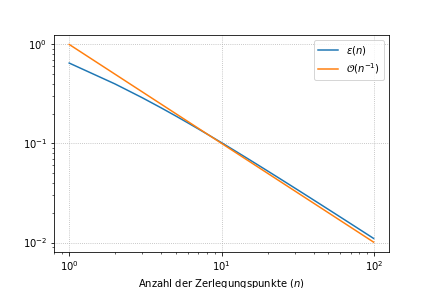
\includegraphics
  [width = 0.5 \textwidth]
  {Fehler zum Endzeitpunkt vs. Anzahl der Zerlegungspunkte}
  \caption{Konvergenzplot}
  \label{Konvergenzplot}
\end{figure}

\end{solution}
